\begin{frame}{From physics to the mathematical model}
  \vspace{-0.6cm}
  \begin{overprint}
    \onslide<1>
    \begin{columns}
      \begin{column}{0.45\textwidth}
        \begin{block}{Solid dynamics problems}
          \begin{itemize}
          \item[] \textbf{Impact; Crash-proof design}
          \item[] High-speed forming
          \item[] Earthquake reliability of structures 
          \end{itemize}
        \end{block}
      \end{column}
      
      \begin{column}{0.55\textwidth}
      \end{column}
    \end{columns}
    
    \begin{figure}[ht]
      \centering
      \subcaptionbox{Bird strike on aircrafts}{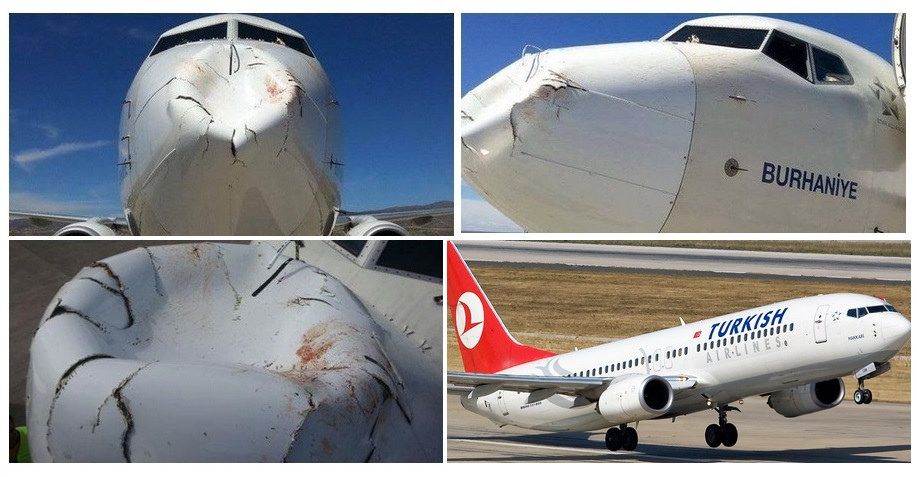
\includegraphics[height=0.3\paperheight]{section1/pictures/birdstrike.jpg}}
      \subcaptionbox{Glasgow Museum of Transport}{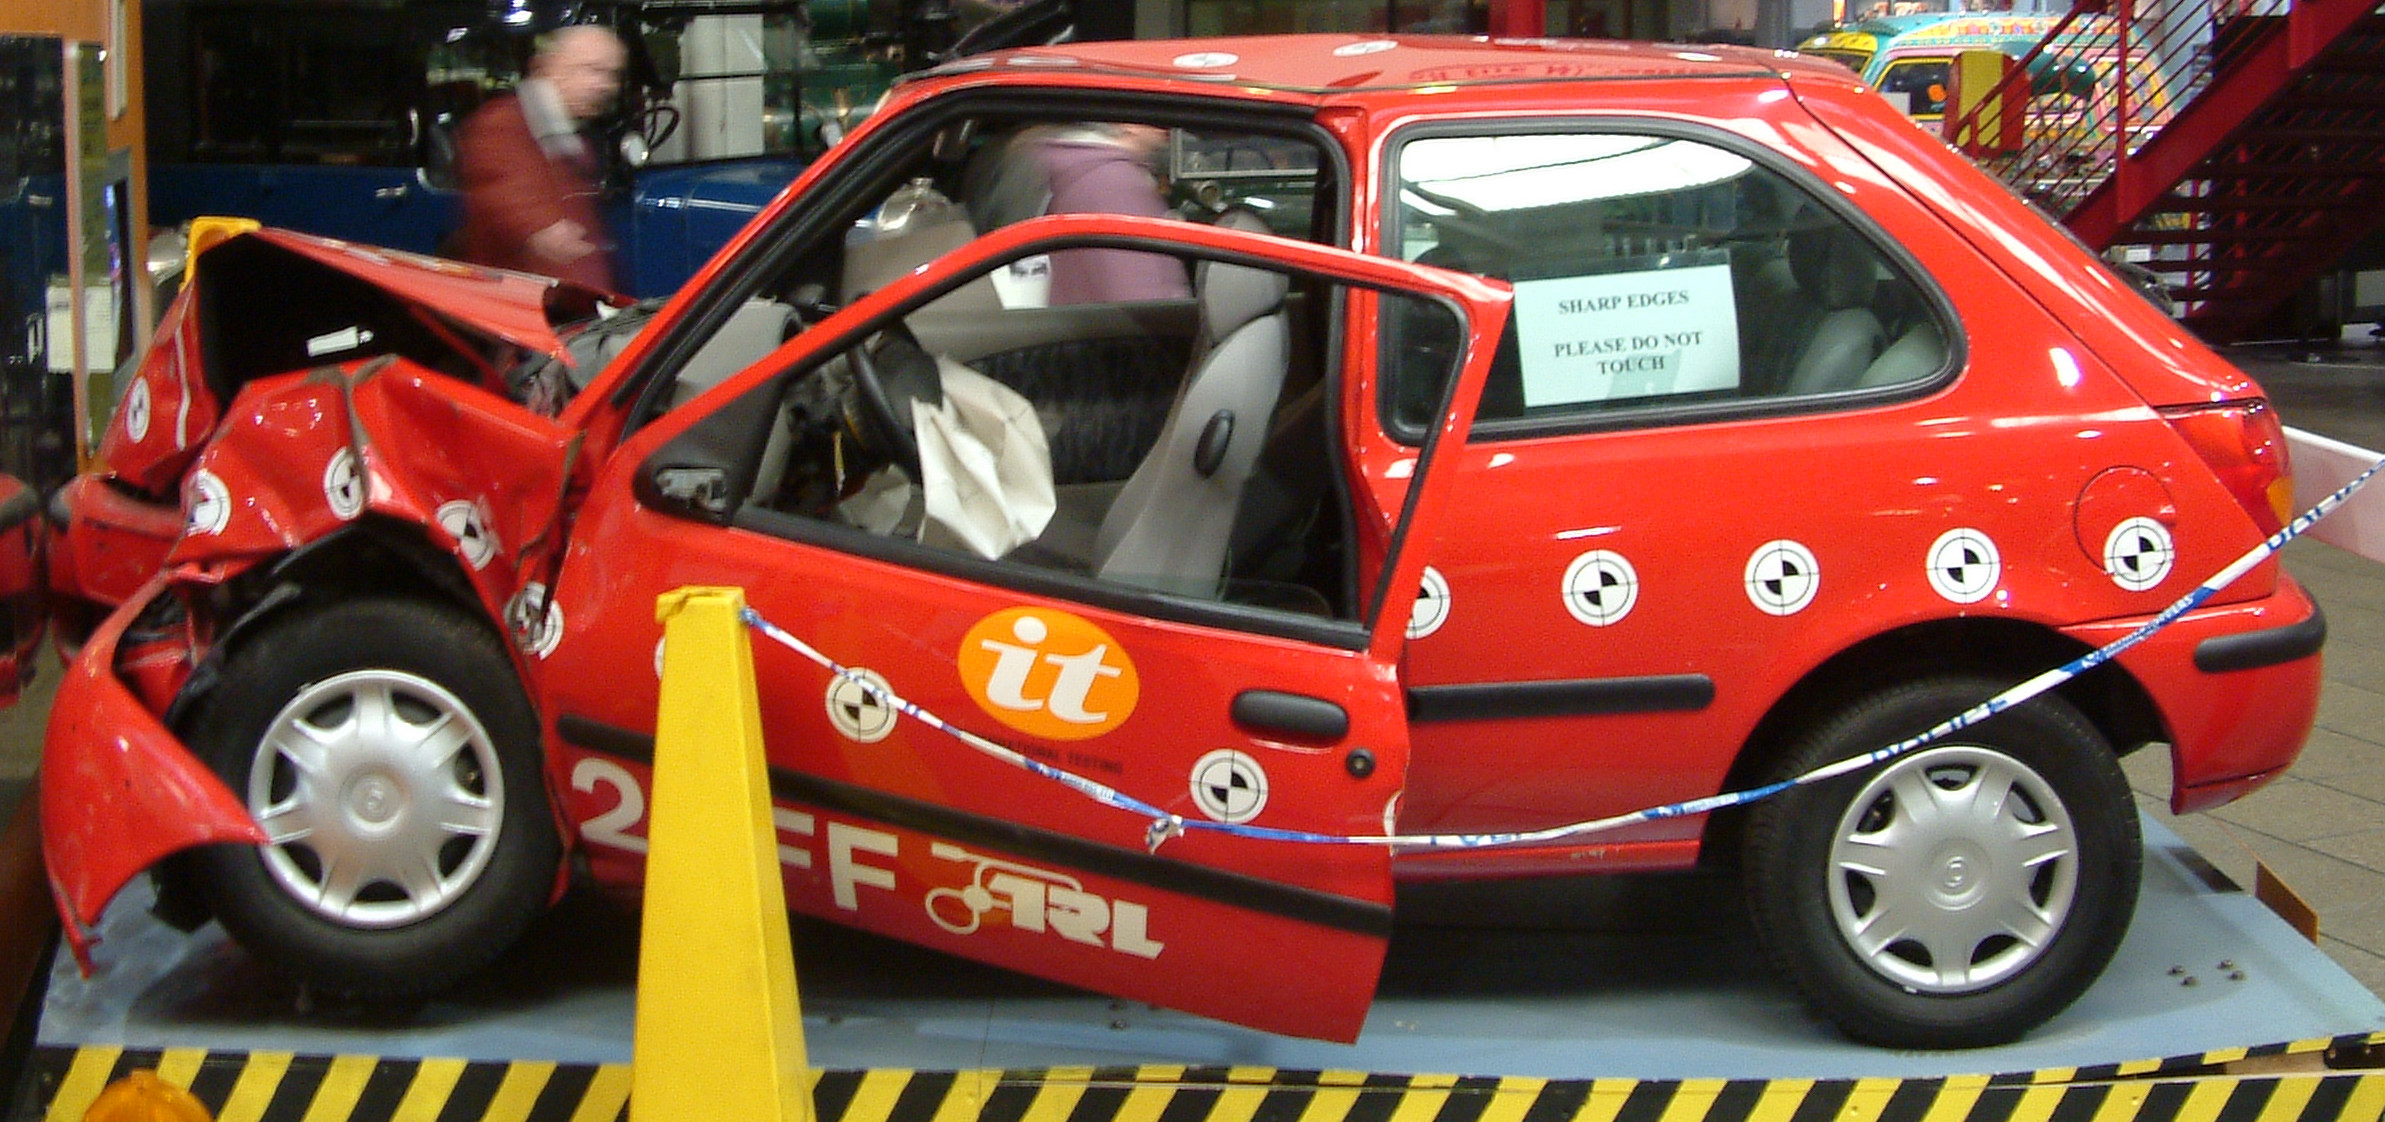
\includegraphics[height=0.3\paperheight]{section1/pictures/crash2.jpg}}
    \end{figure}
    
    \onslide<2>
    \begin{columns}
      \begin{column}{0.45\textwidth}
        \begin{block}{Solid dynamics problems}
          \begin{itemize}
          \item[] Impact; Crash-proof design
          \item[] \textbf{High-speed forming}
          \item[] Earthquake reliability of structures 
          \end{itemize}
        \end{block}
      \end{column}
      
      \begin{column}{0.55\textwidth}
      \end{column}
    \end{columns}

    \centering
    \movie[height = 0.35\paperheight,width=0.25\linewidth,loop,poster,autostart]{}{%
      section1/animation/output3.mp4}\\
    \scriptsize Electromagnetic forming \cite{Formage}
    \vfill
    {\tiny
      \usebibitemtemplate{\color{structure}\insertbiblabel} 
      \usebibliographyblocktemplate{\color{structure}}{\color{black}}{\color{structure!75}}{\color{structure!75}} 
      \begin{thebibliography}{EMF}
        \tiny \bibitem[1]{Formage}
        Bon E.,Priem D.,Sow C., Heuzé T., Racineux G.
        \newblock Electromagnetic bending of an aluminum sheet
        \newblock {\em GeM, Ecole centrale de Nantes, 2015}.
      \end{thebibliography}}  

    \onslide<3>
    \begin{columns}
      \begin{column}{0.45\textwidth}
        \begin{block}{Solid dynamics problems}
          \begin{itemize}
          \item[] Impact; Crash-proof design
          \item[] High-speed forming
          \item[] \textbf{Earthquake reliability of structures}
          \end{itemize}
        \end{block}
      \end{column}
      
      \begin{column}{0.55\textwidth}
      \end{column}
    \end{columns}

    \centering
    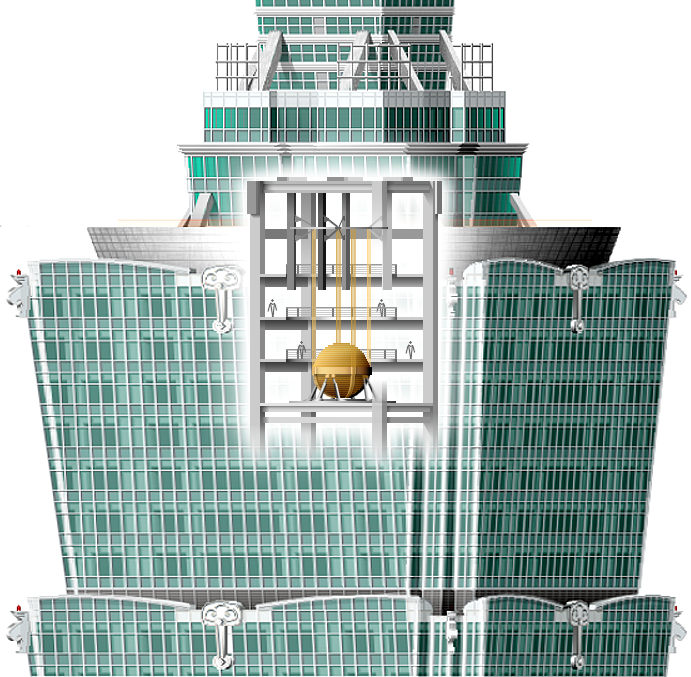
\includegraphics[scale=0.15]{section1/pictures/TaipeiTower.png} \quad
    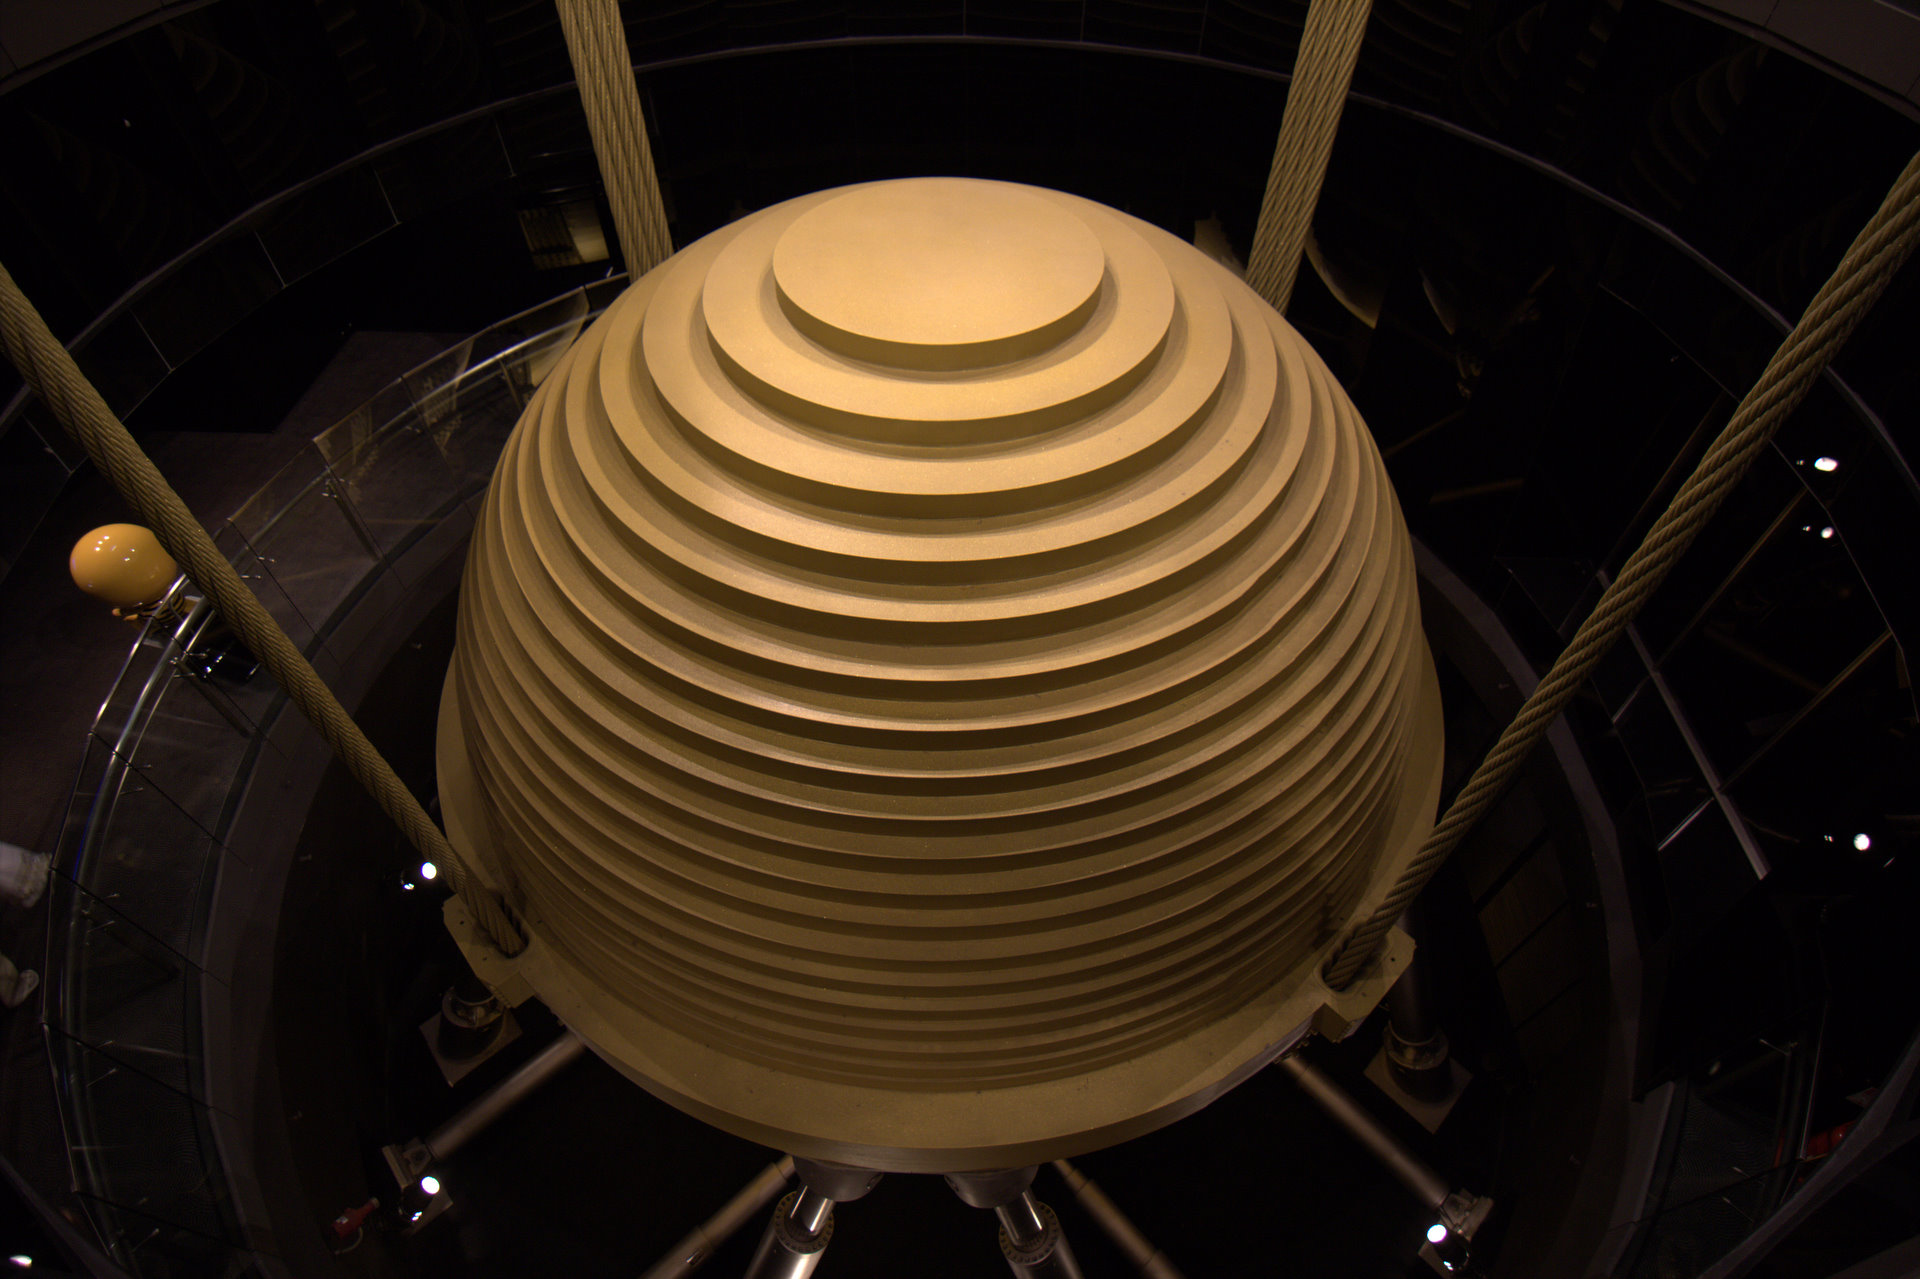
\includegraphics[scale=0.08]{section1/pictures/MassDamper.jpg}\\
    \scriptsize Taipei 101 mass damper

    \onslide<4>
    \begin{columns}
      \begin{column}{0.45\textwidth}
        \begin{block}{Solid dynamics problems}
          \begin{itemize}
          \item[] Impact; Crash-proof design
          \item[] High-speed forming
          \item[] Earthquake reliability of structures 
          \end{itemize}
        \end{block}
      \end{column}
      
      \begin{column}{0.55\textwidth}
        \begin{block}{Partial differential equations}
          \begin{equation*}
            \Rightarrow \left\lvert
              \begin{aligned}
                & \text{Conservation laws} \\
                & \text{Constitutive equations} 
              \end{aligned}
            \right. = \textbf{Hyperbolic system}
            % Préciser les équations dans le dévelopement de la DGMPM
          \end{equation*}
        \end{block}
      \end{column}
    \end{columns}
    
    \begin{block}{Difficulties for the solution of equations:}
      \begin{itemize}
      \item complex geometries
      \item waves propagating/interacting in solids
      \item finite deformations
      \end{itemize}
    \end{block}
    
  \end{overprint}
\end{frame}

% Problems considered -- dynamics + applications + solid mechanics (equations)
% Soit (i) on inclue les équations du modèle dans les motivations soit (ii) on parle d'abord des difficultés qu'après on illustre ?

% (i) - Problèmes de dynamique des solides: lois de conservations + lois constitutives => système hyperbolique
% - EDP dont les solutions font intervenir des ondes
% - Equations complexes (non-linéaires + multi-dimensionnelle) + solutions compliquées car ondes qui interagissent
% - Intérêt de la simulation pour calculer des solutions approchées
% - Mais cependant, on a des limitations (grandes defs ; suivi des ondes [oscillations + diffusion] ; difficultées à assurer la convergence vers une solution physique ??? [un truc pour introduire la prise en compte de la structure caractéristique])
% - Exemples de limitations avec les méthodes existantes : FEM -- FV -- Meshfree 

\begin{frame}{Numerical simulation}
  \begin{block}{It allows to:}
    \begin{itemize}
    \item compute approximate solutions
    \item highlight phenomena implicitly described by the model
    \item perform virtual experiments
    \end{itemize}
  \end{block}
  \metroset{block=fill}
  \begin{block}{Pros and cons of some mesh-based methods:}
    \metroset{block=transparent}
    \begin{scriptsize}
      \begin{columns}
        \begin{column}{.45\textwidth}
          \begin{block}{\scriptsize The Finite Element Method (FEM)}
            \begin{itemize}
            \item[$+$] handle nonlinear constitutive models
            \item[$+$] high-order approximation
            \item[$-$] oscillations near discontinuities
            \item[$-$] dealing with large deformations
            \end{itemize}
          \end{block}
        \end{column}
        \begin{column}{.45\textwidth}
          \begin{block}{\scriptsize The Finite Volume Method (FVM)}
            \begin{itemize}
            \item[$+$] handle nonlinear constitutive models
            \item[$-$] high-order approximation
            \item[$+$] removal of oscillations
            \item[$-$] dealing with large deformations
            \end{itemize}
          \end{block}
        \end{column}
      \end{columns}
    \end{scriptsize}
  \end{block}
  %% Dire que ces méthodes sont basées sur une discretization des domaines spatiaux et temporels
  % \begin{block}{Mainly used methods:}
  %   \metroset{block=transparent}
  %   \begin{columns}
  %     \begin{column}{0.47\textwidth}
  %       \begin{block}{Mesh-based}
  %         \begin{itemize}
  %         \item[] Finite Element Method (FEM)
  %         \item[] Finite Volume Method (FVM)
  %         \end{itemize}
  %       \end{block}
  %     \end{column}
  %     \begin{column}{0.47\textwidth}
  %       \begin{block}{Mesh-free}
  %         \begin{itemize}
  %         \item[] Smooth Particle Hydrodynamics (SPH)
  %         \item[] Particle In Cell methods (PIC)
  %         \end{itemize}
  %       \end{block}
  %     \end{column}
  %   \end{columns}    
  % \end{block}
\end{frame}

\begin{frame}{Numerical simulation}
  \begin{block}{The Discontinuous Galerkin approximation: take advantage of both FEM and FVM}
    \begin{itemize}
    \item[$+$] handle nonlinear constitutive models
    \item[$+$] high-order approximation
    \item[$+$] removal of oscillations
    \item[$-$] dealing with large deformations
    \end{itemize}
  \end{block}

  \begin{block}{Mesh-free methods: Particle in cell approaches}
    \begin{itemize}
    \item[$+$] handle nonlinear constitutive models
    \item[$+$] high-order approximation
    \item[$-$] numerical oscillations and diffusion near discontinuities
    \item[$+$] handle large deformation
    \end{itemize}
  \end{block}
  Fail to mimic the physical behavior due to the lack of information about the structure (talk about dammage, softening, plasticity)
\end{frame}

\subsection*{Objectives and strategy}
\begin{frame}{Objectives}
  Numerical methods able to deal with finite deformation + waves

  Solution of elastoplasticity problems in 2D
\end{frame}

\begin{frame}{Strategy}
  PIC mapping in MPM + DG approx

  Characteristic structure + loading path etc.

  Il faut bien démarquer les deux parties dans le plan de la prez.
\end{frame}


%%% Local Variables:
%%% mode: latex
%%% TeX-master: "../aRenaud"
%%% End:
